% Quality factor estimation on real resonators — conference deck (~20 min)
% Build: make pdf  |  make pdf-notes   (pdfLaTeX; no shell-escape, no minted)
\ifdefined\rdaBeamernotes\else
\documentclass[aspectratio=169,11pt]{beamer}
\fi

\usepackage[T1]{fontenc}
\usepackage{lmodern}
\usepackage{amsmath}
\usepackage{amssymb}
\usepackage{bm}
\usepackage{booktabs}
\usepackage{siunitx}
\usepackage{graphicx}
\usepackage{xcolor}

\graphicspath{{assets/}}

% ---------------------------------------------------------------------------
% Minimal, clean theme (built-in components; palette matches the figures)
% ---------------------------------------------------------------------------
\usetheme{default}
\usefonttheme{professionalfonts}
\setbeamertemplate{navigation symbols}{}
\setbeamertemplate{itemize items}[circle]
\setbeamercovered{transparent}

\definecolor{rdaccent}{HTML}{1F5FBF}
\definecolor{rdaccent2}{HTML}{D1701A}
\definecolor{rdbad}{HTML}{B32020}
\definecolor{rdgood}{HTML}{2E7D4F}
\definecolor{rdink}{HTML}{1A1A1A}
\definecolor{rdmute}{HTML}{5A5A5A}

\setbeamercolor{normal text}{fg=rdink}
\setbeamercolor{structure}{fg=rdaccent}
\setbeamercolor{frametitle}{fg=rdaccent}
\setbeamercolor{title}{fg=rdaccent}
\setbeamercolor{alerted text}{fg=rdbad}
\setbeamercolor{itemize item}{fg=rdaccent}
\setbeamercolor{itemize subitem}{fg=rdaccent2}

\setbeamerfont{frametitle}{series=\bfseries,size=\large}
\setbeamerfont{title}{series=\bfseries,size=\LARGE}
\setbeamerfont{itemize/enumerate body}{size=\small}

% Frame title with a thin accent rule underneath.
\setbeamertemplate{frametitle}{%
  \vspace{0.35em}%
  \begin{beamercolorbox}[wd=\paperwidth,leftskip=0.9em,rightskip=0.9em]{frametitle}%
    \insertframetitle\par%
    \vspace{0.12em}{\color{rdaccent}\hrule height 1pt}%
  \end{beamercolorbox}%
}

% Footline: short title | page number.
\setbeamertemplate{footline}{%
  \hbox{%
    \begin{beamercolorbox}[wd=0.85\paperwidth,ht=2.4ex,dp=1.0ex,leftskip=0.9em]{}%
      {\color{rdmute}\scriptsize LASSO / ring down $Q$ estimation}%
    \end{beamercolorbox}%
    \begin{beamercolorbox}[wd=0.15\paperwidth,ht=2.4ex,dp=1.0ex,rightskip=0.9em]{}%
      \hfill{\color{rdmute}\scriptsize \insertframenumber}%
    \end{beamercolorbox}%
  }%
}

% Common figure helper: leave room below for descriptive bullets.
\newcommand{\slidefig}[2][0.88]{\centering\includegraphics[width=#1\linewidth,height=0.58\textheight,keepaspectratio]{#2}}
\newcommand{\bad}[1]{\textcolor{rdbad}{\textbf{#1}}}
\newcommand{\good}[1]{\textcolor{rdgood}{\textbf{#1}}}
\newcommand{\dft}{\delta\!f\cdot\tau}

% Speaker-notes PDF: slide on top, \note{...} text below (see slides-notes.tex).
\ifdefined\rdaBeamernotes
\usepackage[beamer-notes]{handoutWithNotes}
\pgfpagesuselayout{1 on 1 with notes}
\fi

% ---------------------------------------------------------------------------
\title{Bias in coherent $Q$ fits on drifting resonators}
\subtitle{Quality factor estimation on ring down data from real, drifting resonators}
\author{LASSO / Laboratory of Space Systems \& Optomechanics}
\institute{University of Arizona, College of Optical Sciences}
\date{August 20, 2026}

\begin{document}

% ----- 1. Title -----
\begin{frame}[plain]
  \vspace{0.2em}
  \begin{center}
    {\usebeamerfont{title}\usebeamercolor[fg]{title}\inserttitle}\\[0.3em]
    {\large\color{rdmute}\insertsubtitle}\\[0.8em]
    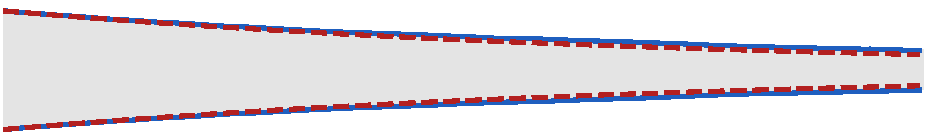
\includegraphics[width=0.78\linewidth]{title-strip.pdf}\\[0.8em]
    
\includegraphics[height=0.9cm,keepaspectratio]{lasso-logo.pdf}\\[0.8em]
    {\small\insertauthor}\\[0.2em]
    {\footnotesize\color{rdmute}\insertinstitute}\\[0.5em]
    {\footnotesize\color{rdmute}Ring down measurements from the ODIN resonators
      \,\textperiodcentered\, \insertdate}
  \end{center}
  \note{\footnotesize
  We estimate the quality factor $Q$ of a mechanical resonator from ring down records:
  excite the mode, release it, fit the free decay, and quote $Q=\pi f\tau$.
  On ODIN engineering development unit (EDU) records, a phase-coherent
  single-exponential fit returned $Q$ biased by up to a factor of four, while quoting a
  95\,\% confidence interval about a part in $10^3$ wide.\\
  This talk is the measurement diagnosis: which model assumptions fail on these data, how
  that bias arises, and which estimator remains usable. Everything shown uses two ring down
  records from the same resonator, taken before and after a vibration test.}
\end{frame}

% ----- 2. The symptom -----
\begin{frame}{Matched-SNR synthetic versus ODIN EDU Pre-Vibe}
  \slidefig[0.96]{symptom-synth-vs-real.pdf}
  \vspace{0.15em}
  \begin{itemize}
    \item Top: oscillating ring down with $\pm$ envelopes implied by a coherent single-$Q$ fit
    \item Bottom: log amplitude (slope $=1/\tau$). Synthetic built at the measured SNR
      ($\approx400$)
    \item Same coherent estimator on both columns: exact on the model, visibly wrong on the
      instrument
  \end{itemize}
  \note{\footnotesize
  \textbf{Ring down:} $A_0e^{-t/\tau}\cos(2\pi ft+\phi)$ with $Q=\pi f\tau$.
  Here $f\approx\SI{7.67}{\hertz}$, $\tau\approx\SI{3700}{\second}$, so $Q\approx9\times10^4$
  and a full decay lasts hours.\\
  The synthetic uses the measured broadband noise ($\approx1.5$ cycles RMS against a
  600-cycle release). Failure on the right is therefore not a low-SNR artifact.}
\end{frame}

% ----- 3. The overlay -----
\begin{frame}{Envelope mismatch on the Pre-Vibe 3\,h window}
  \slidefig[0.92]{overlay-real.pdf}
  \vspace{0.15em}
  \begin{itemize}
    \item Grey points: robust peak-to-peak amplitude (phase-insensitive)
    \item Green: incoherent log-linear slope through those amplitudes
    \item Red dashed: coherent single-frequency exponential; decay rate
      $\approx1.6\times$ too steep
  \end{itemize}
  \note{\footnotesize
  The measured envelope uses $\tfrac12(P_{95}-P_5)$ over 3-cycle windows. It assumes nothing
  about the decay law, so disagreement with the coherent fit is a direct model test.
  On this Pre-Vibe window the coherent $Q$ is about $5.8\times10^4$ while the envelope slope
  gives about $9.4\times10^4$.}
\end{frame}

% ----- 4. Model early -----
\begin{frame}{The fitted model and its three assumptions}
  \slidefig[0.94]{assumptions-card.pdf}
  \vspace{0.15em}
  \begin{itemize}
    \item Every phase-coherent fit on these records assumes this form for hours at a time
    \item Coherent means one fixed $f$ and $\phi$ across the whole window
    \item Broadband SNR $\approx400$: noise alone cannot explain the mismatch on slide~2
  \end{itemize}
  \note{\footnotesize
  Introduce the model as soon as fit results appear. The next slides quantify each
  assumption against the ODIN EDU data. Do not yet quote the measured drifts, $Q(A)$, or
  plateau level; those come from the data slides that follow.}
\end{frame}

% ----- 5. The numbers + traces -----
\begin{frame}{Pre-Vibe and Post-Vibe: numbers and envelopes}
  \begin{columns}[T]
    \begin{column}{0.42\linewidth}
      {\footnotesize
      \begin{tabular}{lrr}
        \toprule
         & \textbf{Pre} & \textbf{Post}\\
        \midrule
        Coherent $Q$          & \bad{58\,141} & \bad{27\,082}\\
        95\,\% interval       & $\pm0.12\,\%$ & $\pm0.08\,\%$\\
        Incoherent ref.\ $Q$  & 92\,584       & 102\,972\\
        \midrule
        Error                 & \bad{$1.6\times$} & \bad{$3.8\times$}\\
        \bottomrule
      \end{tabular}}
      \vspace{0.6em}
      \begin{itemize}
        \item Interval width measures curvature under the assumed model
        \item It does not test whether that model is adequate
      \end{itemize}
    \end{column}
    \begin{column}{0.56\linewidth}
      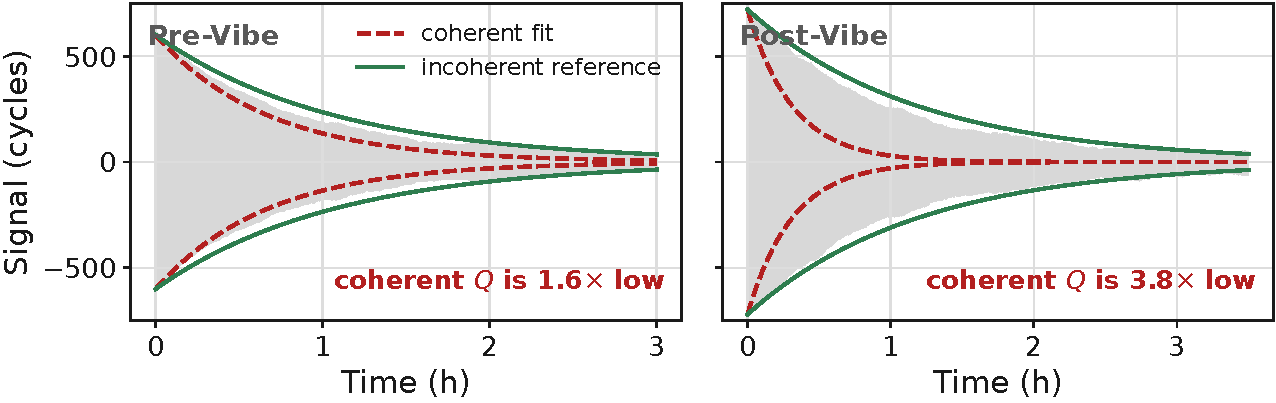
\includegraphics[width=\linewidth,height=0.62\textheight,keepaspectratio]{pre-post-traces.pdf}
    \end{column}
  \end{columns}
  \note{\footnotesize
  Same resonator, same coherent single-exponential estimator, before and after vibration.
  Red envelopes use the coherent $Q$; green envelopes use the segmented incoherent
  reference. The confidence interval collapses with $N\sim10^6$ samples whether or not the
  model is right: it bounds variance, not misspecification bias.}
\end{frame}

% ----- 6. Window sensitivity -----
\begin{frame}{Window start and duration dependence of coherent $Q$}
  \slidefig[0.94]{window-sweep-before.pdf}
  \vspace{0.1em}
  \begin{itemize}
    \item Starts at 0, 20, 40, 60, 80, 100\,s (early, high-SNR release); durations 1--6\,h
    \item Pre-Vibe coherent $Q$ scatters by $\approx16\times$ relative to the incoherent reference
    \item Post-Vibe is tighter but systematically low (median $\approx0.29\times$ reference)
  \end{itemize}
  \note{\footnotesize
  Grey band: genuine $Q(A)$ range measured later; no single-$Q$ estimator should be blamed
  for lying inside it. The scatter outside that band is the estimator failure.
  Irreproducibility at float round-off for a fixed window is shown on the crop-cascade slide,
  where two selections of the same Post-Vibe segment differ only in the last bits of the
  inputs yet crop to 107\,s versus 3154\,s.}
\end{frame}

% ----- 7. Violation 1 -----
\begin{frame}{Assumption 1: frequency is not constant during the decay}
  \slidefig[0.96]{drift-pull.pdf}
  \vspace{0.1em}
  \begin{itemize}
    \item Left: ideal synthetic (matched Pre-Vibe SNR/$Q$) stays flat in $f$ vs amplitude
    \item Middle/right: ODIN EDU $f$ rises $+1.2$\,mHz (Pre) and $+0.2$\,mHz (Post) as $A$ falls
    \item Linear in $\log A$: anharmonic pull, not a slow thermal drift
  \end{itemize}
  \note{\footnotesize
  Per-segment tone fits (120\,s) measure $f(t)$ without committing to a full-record coherent
  model. A 1\,mHz frequency error accumulates one cycle of phase slip in about 1000\,s; fit
  windows here are several hours.}
\end{frame}

% ----- 8. Violation 2 -----
\begin{frame}{Assumption 2: the decay is not a single exponential}
  \slidefig[0.96]{q-vs-amplitude.pdf}
  \vspace{0.1em}
  \begin{itemize}
    \item Left: synthetic residual of a one-$\tau$ fit is consistent with noise
    \item Middle: ODIN EDU residual shows smooth curvature well above segment scatter
    \item Right: local Pre-Vibe $Q$ runs $\approx7\times10^4$ to $1.8\times10^5$ with amplitude
  \end{itemize}
  \note{\footnotesize
  Amplitude-dependent damping means there is no single true $Q$ for the whole decay. A window
  choice selects an amplitude-weighted average. Nonlinear least squares weights early
  high-amplitude samples; a log-envelope fit weights used windows more evenly, so the two
  can disagree without either fit being numerically broken.}
\end{frame}

% ----- 9. Violation 3 -----
\begin{frame}{Assumption 3: the amplitude does not decay to the noise floor}
  \slidefig[0.96]{plateau.pdf}
  \vspace{0.1em}
  \begin{itemize}
    \item Left: synthetic decays into the broadband noise floor
    \item Middle: both EDU records settle near 17 cycles with nulls and revivals
    \item Right: plateau spectrum still shows the analysis tone (narrowband drive)
  \end{itemize}
  \note{\footnotesize
  The plateau is coherent signal at the analysis frequency, roughly ten times the broadband
  RMS, so filtering cannot separate it from the ring down. An explicit amplitude-floor term
  is required in the envelope model.}
\end{frame}

% ----- 10. Model revisited -----
\begin{frame}{Same model, now with the measured violations}
  \slidefig[0.94]{assumptions-card-late.pdf}
  \vspace{0.15em}
  \begin{itemize}
    \item Frequency pull and $Q(A)$ are resonator physics: report them, do not average them away
    \item The driven plateau is a fitting nuisance: model it as an amplitude floor
    \item Two of three failures are measurements; one is an analysis contaminant
  \end{itemize}
  \note{\footnotesize
  Explicit mapping: (1) anharmonic pull and (2) amplitude-dependent damping are physics worth
  publishing as $f(A)$ and $Q(A)$. (3) Ambient drive that pins a late-time plateau biases
  long-window envelope slopes and must be handled as a floor, not as ``more noise''.}
\end{frame}

% ----- 11. Injection -----
\begin{frame}{Controlled injection: one measured pathology at a time}
  \slidefig[0.94]{injection-ladder.pdf}
  \vspace{0.1em}
  \begin{itemize}
    \item Base record: ideal synthetic at Pre-Vibe $f_s$, $f_0$, $\tau$, $A_0$, and noise
    \item Red: coherent single-$f$ $Q$/truth after each injection; green: segmented demodulation
    \item Injecting only the measured Pre-Vibe $f(t)$ spans $0.51\times$ to $3.80\times$ of truth
  \end{itemize}
  \note{\footnotesize
  Nothing injected recovers truth for every estimator (noise exonerated by construction).
  Amplitude-proportional pull and plain linear drift each break the coherent fit by
  $1.6$--$1.9\times$. The measured frequency trajectory alone reproduces the field failure,
  including sensitivity to $\tau$ initialization. The plateau leaves coherent fits nearly
  unbiased (phase averages) but pulls the envelope high.}
\end{frame}

% ----- 12. Coherence budget -----
\begin{frame}{Coherence budget: $\dft \lesssim 0.01$ for percent-level bias}
  \slidefig[0.90]{coherence-budget.pdf}
  \vspace{0.1em}
  \begin{itemize}
    \item Scan a fixed frequency error on the ideal synthetic; plot $Q/Q_{\rm true}$ vs $\dft$
    \item Bias under 2\,\% needs $f$ stable to $\approx\SI{3}{\micro\hertz}$ at $\tau\approx\SI{3700}{\second}$
    \item EDU drifts $300$--$1100\,\mu$Hz: $\dft\sim\mathcal{O}(1)$, far past the knee
  \end{itemize}
  \note{\footnotesize
  $\dft$ is the accumulated phase error over the information-carrying decay time. Above
  $\approx0.01$, coherent single-frequency fitting is not recoverable by a better optimizer
  or a better constant-$f$ seed: no single frequency is correct across the window.}
\end{frame}

% ----- 13. Crop cascade -----
\begin{frame}{Secondary failure: a collapsed $\tau$ silently crops the window}
  \slidefig[0.92]{crop-cascade.pdf}
  \vspace{0.1em}
  \begin{itemize}
    \item Analysis used $3\tau_{\rm seed}$ as the fit window; a bad seed shrinks the data
    \item Same 3.5\,h Post-Vibe segment, inputs differing at float round-off:
      $\tau=36$\,s (crop 107\,s) vs $\tau=1051$\,s (crop 3154\,s)
    \item An independent envelope $\tau\approx5700$\,s was available and unused
  \end{itemize}
  \note{\footnotesize
  This is the round-off lottery made visible: identical sample count and span, last-bit input
  changes, two near-degenerate minima. Design rule: never let a fitted parameter silently
  choose the analysis window; cross-check against an independent amplitude-based $\tau$.}
\end{frame}

% ----- 14. The fix -----
\begin{frame}{Estimator that survives these records: segmented demodulation}
  \slidefig[0.90]{demod-method.pdf}
  \vspace{0.1em}
  \begin{columns}[T]
    \begin{column}{0.5\linewidth}
      \begin{itemize}
        \item Coherent tone fit inside each short segment only
        \item Explicit amplitude floor for the driven plateau
      \end{itemize}
    \end{column}
    \begin{column}{0.48\linewidth}
      \begin{itemize}
        \item Robust log-envelope slope (Theil--Sen) on $A>3A_{\rm floor}$
        \item Report $Q$ versus amplitude; bootstrap uncertainties
      \end{itemize}
    \end{column}
  \end{columns}
  \note{\footnotesize
  Phase must hold for $\sim$120\,s, not for hours. Floor correction removes the plateau from
  the slope fit. Amplitude bands expose $Q(A)$ instead of forcing one average. Controlled
  experiments (including injected measured drift) stay within 2\,\% of truth.}
\end{frame}

% ----- 15. Adequacy checks -----
\begin{frame}{Model-adequacy checks before quoting a finite $Q$}
  \slidefig[0.92]{gates-flow.pdf}
  \vspace{0.1em}
  \begin{itemize}
    \item Refuse plateau-dominated windows (no usable free decay)
    \item Prefer incoherent $Q$ when $\dft$ is large; keep coherent $Q$ only if coherence holds
    \item Require coherent and incoherent estimates to agree within $1.5\times$, else no number
  \end{itemize}
  \note{\footnotesize
  The useful output on inadequate data is a refusal. Each check uses measured diagnostics
  (dynamic range, coherence ratio, cross-estimator agreement), not merely optimizer
  convergence.}
\end{frame}

% ----- 16. Validation -----
\begin{frame}{After the change: window sweep against the same reference}
  \slidefig[0.94]{window-sweep-after.pdf}
  \vspace{0.1em}
  \begin{itemize}
    \item Pre-Vibe coherent-fit spread of $\approx16\times$ falls to $\approx1.3\times$ under segmented
      demodulation; residual start/duration dependence is $Q(A)$, not instability
    \item Surviving windows fall inside the physical $Q(A)$ band
    \item Plateau-dominated windows return no finite $Q$ (marked on the axis floor)
  \end{itemize}
  \note{\footnotesize
  Pre-Vibe coherent-fit spread of $\approx16\times$ falls to about $1.3\times$ under segmented
  demodulation. Short early windows sample the low-$Q$, high-amplitude part of the decay, so
  some residual start/duration dependence remains and should be read as $Q(A)$, not as
  instability.}
\end{frame}

% ----- 17. Payoff -----
\begin{frame}{Pre/Post vibration comparison at matched amplitude}
  \slidefig[0.92]{pre-post.pdf}
  \vspace{0.1em}
  \begin{itemize}
    \item Single-number coherent fits had suggested $\sim$30\,\% $Q$ loss after vibe
    \item Amplitude-matched demodulation: Post-Vibe $Q$ equal or higher in every band
    \item What changed: $f$ down 77--140\,ppm; pull coefficient weaker by $\approx5\times$
  \end{itemize}
  \note{\footnotesize
  When $Q$ depends on amplitude, compare only at matched amplitude with matched segmentation.
  Otherwise two different window averages are mistaken for a physical change. Loss did not
  degrade; the nonlinearity did change.}
\end{frame}

% ----- 18. Takeaways -----
\begin{frame}[c]{Practical rules, and what remains open}
  \begin{columns}[T]
    \begin{column}{0.54\linewidth}
      {\color{rdaccent}\textbf{Take these home}}
      \vspace{0.4em}
      \begin{itemize}
        \item Test model adequacy, not only fit convergence
        \item Compute $\dft$ from short segments before a coherent fit
        \item If $Q$ depends on $A$, report $Q(A)$ (or the law), not one number
      \end{itemize}
    \end{column}
    \begin{column}{0.44\linewidth}
      {\color{rdmute}\textbf{Still open}}
      \vspace{0.4em}
      \begin{itemize}
        \item Microscopic origin of pull and damping
        \item Source of the ambient drive
        \item One EDU pair so far, not a survey
      \end{itemize}
    \end{column}
  \end{columns}
  \vspace{1.4em}
  \begin{beamercolorbox}[wd=\textwidth,center,rounded=true,shadow=false]{}
    {\large\color{rdbad}\textbf{A tight interval under a wrong model is worse than no
    interval.}}
  \end{beamercolorbox}
  \note{\footnotesize
  Invite others to compute $\dft$ on their own ring downs. If it is not $\lesssim0.01$, a
  published coherent $Q$ may be window- and initialization-dependent in the same way.}
\end{frame}

% ===========================================================================
\appendix

\begin{frame}{Backup: why not fit a drifting phase and stay coherent?}
  \[
    x(t)=A_0e^{-t/\tau}\cos\!\Big(2\pi\!\int_0^t\! f(t')\,dt' + \phi\Big)+c
  \]
  \vspace{0.2em}
  \begin{itemize}
    \item Possible in principle with a polynomial or spline phase
    \item At SNR $\approx400$, information gain over incoherent demodulation is small
    \item Extra phase parameters worsen an already near-degenerate objective
    \item Prony, matrix pencil, and linewidth fits inherit a constant-frequency pole
  \end{itemize}
  \vfill
  \note{\footnotesize
  A flexible phase model can absorb the measured trajectory, but it does not beat segmented
  demodulation here and reintroduces the lottery among near-degenerate minima.}
\end{frame}

\begin{frame}{Backup: multi-mode and beating ruled out}
  \vfill
  \slidefig[0.92]{backup-spectra.pdf}
  \begin{itemize}
    \item One dominant peak, 7.669--7.672\,Hz on both records
    \item Nearest features $\sim10^5\times$ weaker, consistent with leakage of a drifting tone
  \end{itemize}
  \vfill
  \note{\footnotesize
  Beating from a nearby mode would mimic non-exponential decay. Spectra of decay and plateau
  segments show a single dominant line, so the curvature on the $Q(A)$ slide is damping
  physics, not modal interference.}
\end{frame}

\begin{frame}{Backup: why a curvature interval collapses}
  \[
    \nu\log\frac{\mathrm{RSS}(\tau)}{\mathrm{RSS}_{\min}}\le\chi^2_{0.95,1},
    \qquad \nu=N-p,\quad N\sim10^6
  \]
  \vspace{0.2em}
  \begin{itemize}
    \item Width scales as $1/\sqrt{N}$ under the assumed white-noise model
    \item Bounds variance; contains no misspecification term
    \item Residuals here are not white: the plateau is narrowband
  \end{itemize}
  \vfill
  \note{\footnotesize
  The profile interval is correct on its own model and remains appropriate for short,
  coherent records. It is the wrong default for multi-hour EDU decays without an adequacy
  test.}
\end{frame}

\begin{frame}{Backup: residual window spread after the fix}
  \slidefig[0.88]{window-sweep-after.pdf}
  \begin{itemize}
    \item Short early windows sample the low-$Q$, high-amplitude part of the decay
    \item Residual $\approx1.3\times$ spread sits inside the measured $Q(A)$ band
  \end{itemize}
  \vfill
  \note{\footnotesize
  Re-estimating per window exposes physical $Q(A)$. Forcing a tighter window-stability
  number would hide amplitude dependence that should be reported.}
\end{frame}

\begin{frame}{Backup: Theil--Sen versus least squares on the log envelope}
  \begin{itemize}
    \item Theil--Sen: median of pairwise slopes; resistant to plateau revivals
    \item Least squares: 5--10\,\% higher $Q$ on these curved decays
    \item Difference is driven by curvature weighting, not by noise
  \end{itemize}
  \vfill
  \note{\footnotesize
  Robust regression was chosen because a single revival inside the fit region pulls a
  least-squares slope. The offset relative to least squares is left visible rather than
  tuned away.}
\end{frame}

\begin{frame}{Backup: records and conventions}
  \centering
  \begin{tabular}{lrr}
    \toprule
     & \textbf{Pre-Vibe} & \textbf{Post-Vibe}\\
    \midrule
    Record length            & \SI{28350}{\second} & \SI{62176}{\second}\\
    Sample rate              & \SI{149.012}{\hertz} & \SI{149.012}{\hertz}\\
    Mean frequency           & \SI{7.6704}{\hertz} & \SI{7.6694}{\hertz}\\
    Release amplitude        & $\approx600$ cycles & $\approx600$ cycles\\
    Broadband noise          & 1.3 cycles RMS & 1.9 cycles RMS\\
    Plateau amplitude        & 16.3 cycles & 17.1 cycles\\
    Drift over decay         & $+1.19$ mHz & $+0.22$ mHz\\
    Segmented $Q$ (matched)  & $9.08\times10^4$ & $9.37\times10^4$\\
    \bottomrule
  \end{tabular}
  \vspace{0.8em}
  \parbox{0.92\textwidth}{\centering\footnotesize\color{rdmute}$Q=\pi f\tau$; amplitudes in
  phasemeter cycles; matched protocol: \SI{120}{\second} segments over a common
  \SI{21600}{\second} window}
  \note{\footnotesize
  Both records are interferometric phasemeter exports of the same ODIN EDU resonator,
  before and after vibration, with the same excitation and readout.}
\end{frame}

\end{document}
